\documentclass[12pt,a4paper]{article}
\usepackage[utf8]{inputenc}
%Set page layout parameters
\usepackage[
	top=4cm,
	bottom=2cm,
	left=2cm,
	right=2cm,
	headheight=2cm,
	footskip=1cm,
	marginparwidth=2cm]{geometry}
\usepackage[dvipsnames]{xcolor}
% To use color boxes
\usepackage{tcolorbox}
\usepackage{lipsum}
\tcbuselibrary{listings,theorems,skins,vignette,raster,breakable,magazine,poster,fitting,hooks}
\newcounter{ejemplo}
%Images path
\graphicspath{{images/}}
\usepackage{float} %provide us with the option H
\usepackage{fancyhdr}
\usepackage{tikz}
\usepackage{tikzpagenodes}
%to redefine figure caption 
\renewcommand{\figurename}{Figura}
%change text font
\usepackage[T1]{fontenc}
\usepackage{tgbonum} % LaTeX will use the TEX Gyre Bonum font family

\definecolor{subtitle_yellow}{RGB}{252,213,129}
\definecolor{title_yellow}{RGB}{249,175,16}
\definecolor{steel_blue_title}{RGB}{93,138,168}
\definecolor{pewter_blue_subtitle}{RGB}{149,178,198}
\definecolor{ecru_circle}{RGB}{215,190,130}
\definecolor{ecru_circle1}{RGB}{68,148,173}

\newcommand{\myfirststyle}{%
	\begin{tikzpicture}[remember picture, overlay]
		
		%top border
		\fill[fill=steel_blue_title](current page.north west) rectangle ([yshift=-15mm]current page.north east);
		
		\fill[fill=pewter_blue_subtitle]([yshift=-17mm]current page.north west) rectangle ([yshift=-30mm]current page.north east);
		
		%page box
		%\draw[lightgray, fill=Rhodamine, fill opacity=0.05, line width=1mm, rounded corners=3mm] ([xshift=-5mm,yshift=5mm]current page text area.north west) rectangle ([xshift=5mm,yshift=-5mm]current page text area.south east);
		
		%bottom box
		\fill[fill=pewter_blue_subtitle](current page.south west) rectangle ([yshift=10mm]current page.south east);
		
		%page circle
		\draw[white,fill=ecru_circle1,line width=2mm] ([xshift=-5mm,yshift=25mm]current page text area.north east) circle (1); 
		
		
		%page number text        
		%\node[anchor=center] at ([xshift=-5mm,yshift=25mm]current page text area.north east) {\Huge\bfseries\sffamily\color{white}{\thepage}};
		
		%title text
		\node[anchor=west] at ([yshift=32mm]current page text area.north west) {\Huge\bfseries\sffamily\color{white}{Resistores en serie}};
		
		%subtitle text
		\node[anchor=west] at ([xshift=10mm,yshift=16mm]current page text area.north west) {\Large\bfseries\sffamily\color{white}{Divisor de tensión}};
		
		%footer text
		\node[anchor=center] at ([yshift=-15mm]current page text area.south) {\large\bfseries\sffamily\color{white}{Created by: Rodrigo Castillejos}};
		
	\end{tikzpicture}
}


%create page style
\fancypagestyle{MyFirstStyle}{%
	\fancyhf{}
	\fancyhead[C]{\myfirststyle}
	\renewcommand{\headrulewidth}{0pt}
}%

\pagestyle{MyFirstStyle}

\colorlet{colexam}{red!75!black}
\newtcolorbox[use counter=ejemplo]{myexample}{%
	empty,title={Ejemplo \thetcbcounter},attach boxed title to top left,
	boxed title style={empty,size=minimal,toprule=2pt,top=4pt,
		overlay={\draw[colexam,line width=2pt]
			([yshift=-1pt]frame.north west)--([yshift=-1pt]frame.north east);}},
	coltitle=colexam,fonttitle=\Large\bfseries,
	before=\par\medskip\noindent,parbox=false,boxsep=0pt,left=0pt,right=3mm,top=4pt,
	breakable,pad at break*=0mm,vfill before first,
	overlay unbroken={\draw[colexam,line width=1pt]
		([yshift=-1pt]title.north east)--([xshift=-0.5pt,yshift=-1pt]title.north-|frame.east)
		--([xshift=-0.5pt]frame.south east)--(frame.south west); },
	overlay first={\draw[colexam,line width=1pt]
		([yshift=-1pt]title.north east)--([xshift=-0.5pt,yshift=-1pt]title.north-|frame.east)
		--([xshift=-0.5pt]frame.south east); },
	overlay middle={\draw[colexam,line width=1pt] ([xshift=-0.5pt]frame.north east)
		--([xshift=-0.5pt]frame.south east); },
	overlay last={\draw[colexam,line width=1pt] ([xshift=-0.5pt]frame.north east)
		--([xshift=-0.5pt]frame.south east)--(frame.south west);},%
}


\begin{document}
	Considérese el circuito de un solo lazo de la figura \ref{fig:pic1}. Los dos resistores están en serie, ya que en ambos fluye la misma corriente $i$. Al aplicar la ley de Ohm en cada uno de los resistores se obtiene:
	
	\begin{figure}[H]
		\centering
		
\includegraphics[scale=0.5]{figure1}
		\caption{Divisor de tensión con dos resistores.}
		\label{fig:pic1}
	\end{figure}

	\begin{align}
		\label{E:eq1}
		v_1 = iR_1 && v_2 = iR_2
	\end{align}
	
	Si se aplica la LTK al lazo de la figura \ref{fig:pic1} (desplazándose en el sentido de las manecillas del reloj), se tiene
	
	\begin{align}
		\label{E:eq2}
		-v+v_1+v_2=0
	\end{align}
	
	Despejando $v$ de la ecuación (\ref{E:eq2}) obtenemos
	
	\begin{align}
		\label{E:eq3}
		v=v_1+v_2
	\end{align}

	De la combinación de la ecuación (\ref{E:eq1}) y de la ecuación (\ref{E:eq3}) obtenemos 
	
	\begin{align}
		\label{E:eq4}
		v = iR_1+iR_2 = i(R_1+R_2)
	\end{align}

	O sea
	
	\begin{align}
		\label{E:eq5}
		i = \frac{v}{R_1+R_2}
	\end{align}
	
	Nótese que la ecuación (\ref{E:eq4}) puede escribirse como
	\begin{align}
		\label{E:eq6}
		v = i(R_{eq})
	\end{align}
	
	Lo que implica que los resistores pueden reemplazarse por un resistor equivalente $R_{eq}$, esto es
	\begin{align}
		\label{E:eq7}
		R_{eq} = R_1 + R_2
	\end{align}
	
	Así la figura \ref{fig:pic1} puede reemplazarse por el circuito equivalente de la figura \ref{fig:pic2}. En general
	
	\begin{tcolorbox}
		La resistencia equivalente de cualquier número de resistores conectados en serie es la suma de las resistencias individuales.
	\end{tcolorbox}

	\begin{figure}[H]
		\centering
		
\includegraphics[scale=0.5]{figure2}
		\caption{Circuito equivalente.}
		\label{fig:pic2}
	\end{figure}
	
	Así, en el caso de $N$ resistores en serie
	\begin{tcolorbox}[colback=red!5!white,colframe=red!75!black]
		\begin{equation}
			\label{E:eq8}
			R_{eq} = R_1 + R_2 + \dotsb + R_N = \sum_{n=1}^{N} R_n 
		\end{equation}
	\end{tcolorbox}
	
	Para determinar la tensión a lo largo de cada resistor de la figura \ref{fig:pic1}, se sustituye la ecuación (\ref{E:eq5}) en la ecuación (\ref{E:eq1}) 
	\begin{align}
		\label{E:eq9}
		v_1 = \frac{R_1}{R_1 + R_2} v && v_2 = \frac{R_2}{R_1 + R_2} v
	\end{align}
	
	En general, si un divisor de tensión tiene $R$ resistores en serie con una tensión de fuente $v$, el $n$-ésimo resistor $(R_n)$ tendrá una caída de tensión de
	\begin{tcolorbox}[colback=red!5!white,colframe=red!75!black]
		\begin{equation}
			\label{E:eq10}
			v_n = \frac{R_n}{R_1+R_2+\dotsb+R_N}v 
		\end{equation}
	\end{tcolorbox}
	
	\newpage

	\begin{myexample}
		La entrada de un IC requiere 5V constantes, pero la fuente de voltaje es de 9V. Diseñe un divisor de voltaje capaz de crear una salida de 5V. Asuma que el IC tiene una alta resistencia de entrada $(10M\Omega)$ por lo que prácticamente no fluye corriente desde el divisor.
		\begin{figure}[H]
			\centering
			
\includegraphics[scale=0.5]{figure3}
			\caption{Circuito propuesto para el ejemplo1.}
			\label{fig:pic3}
		\end{figure}	
		
		Ya que asumimos que no fluye corriente por el IC, podemos aplicar directamente la ecuación (\ref{E:eq9})
		\begin{align}
			V_o = \frac{R_2}{R_1+R_2}V_{in}\nonumber
		\end{align}
		 
		 Debemos escoger los valores de los resistores de manera que no fluya demasiada corriente por ellos, para así no causar pérdidas de potencia innecesarias. Supongamos que queremos que por el divisor fluya una corriente $i=100\mu A$, así, de la ecuación \ref{E:eq6} tenemos
		 
		 \begin{align}
		 	R_{eq} = \frac{V_{in}}{I_T} = \frac{9V}{100\times 10^{-6}A} = 90k\Omega \nonumber
		 \end{align}
		 
		 Es decir, nuestra combinación de resistencias $R_1+R_2$ debe ser de $90k\Omega$, así, de la ecuación (\ref{E:eq7})
		 
		 \begin{equation}
		 	R_{eq}= R_1 + R_2 = 90k\Omega \nonumber
		 \end{equation}
		 
		 Ahora, si despejamos $R_1$ de la ecuación (\ref{E:eq9}) obtenemos
		 \begin{align}
		 	\label{E:eq11}
		 	\frac{R2}{R_1 + R_2} &= \frac{V_o}{V_{in}}\nonumber\\
		 	R_2V_{in} &= R_1 V_o + R_2 V_o\nonumber \\
		 	R_1 V_o &= (V_{in} - V_o)R_2\nonumber \\\nonumber\\
		 	R1 = \frac{V_{in}-V_o}{V_o} R_2
		 \end{align}
	 
	 	Sin embargo
	 	\begin{equation}
	 		\label{E:eq12}
	 		R_2 = R_{eq} - R_1
	 	\end{equation}
 		
 		Sustituyendo la ecuación (\ref{E:eq12}) en la ecuación (\ref{E:eq11}) obtenemos
 		\begin{align}
 			\label{E:eq13}
 			R_1 &= \left( \frac{V_{in}-V_o}{V_o} \right) \left( R_{eq} - R_1 \right)  \nonumber \\
 			   &= \left( \frac{V_{in}-V_o}{V_o} \right)R_{eq} - \left( \frac{V_{in}-V_o}{V_o} \right)R_1\nonumber \\
 			\left( 1 + \frac{V_{in} - V_o}{V_o} \right) R_1 &= R_{eq} \left( \frac{V_{in}-V_o}{V_o} \right) \nonumber \\
 			\left( \frac{V_{in} - V_o + V_o}{V_o} \right) R_1 &= R_{eq} \left( \frac{V_{in}-V_o}{V_o} \right)\nonumber \\
 			\left( \frac{V_{in}}{V_o}  \right)R_1 &= R_{eq} \left( \frac{V_{in}-V_o}{V_o} \right)\nonumber \\
 			R_1 &= \left( \frac{V_{in} - V_o}{V_{in}}  \right)R_{eq}
 		\end{align}
 		
 		La sustitución de la ecuación (\ref{E:eq13}) y la ecuación (\ref{E:eq12}) por sus valores numéricos da
 		
 		\begin{equation}
 			R_1 = \left( \frac{9V-5V}{9V} \right)(90K\Omega) = 40k\Omega \nonumber
 		\end{equation}
 	
 		Y 
 		\begin{equation}
 			R_2 = R_{eq} - R_1 = 90k\Omega - 40k\Omega = 50k\Omega \nonumber
 		\end{equation}
 		
 		\begin{figure}[H]
 			\centering
 			
\includegraphics[scale=0.7]{figure4}
 			\caption{Simulación del circuito para el ejemplo 1.}
 			\label{fig:pic4}
 		\end{figure}
 		
	\end{myexample}

	\begin{myexample}
		Se tiene una fuente de 10V, pero en el divisor de tensión se conecta un dispositivo que se alimenta a 3V y requiere 9.1mA. Diseñe un divisor de tensión capaz de alimentar dicha carga.
		\begin{figure}[H]
			\centering
			
\includegraphics[scale=1]{figure5}
			\caption{Circuito propuesto para el ejemplo 2.}
			\label{fig:pic5}
		\end{figure}
		
		Para este ejemplo utilizaremos la regla del 10 por ciento. Esta regla es un método estándar para seleccionar $R_1$ y $R_2$ tomando en cuenta la carga y así minimizar las pérdidas de potencia innecesarias en el divisor.
		
		El primer paso es seleccionar $R_2$ de tal manera que $I_2$ sea el 10\% de la corriente de carga, así
		
		\begin{equation}
			I_2 = (0.1)(9.1\times 10^{-3}A) = 0.91mA \nonumber
		\end{equation}
	
		Usamos la ley de Ohm para encontrar la resistencia $R_2$
		\begin{equation}
			R_2 = \frac{3V}{0.91\times 10^{-3}A} = 3297\, \Omega \nonumber
		\end{equation}
		
		Considerando la tolerancia y los valores de resistencia estándar, seleccionamos un resistor de $3300\, \Omega$. Ahora necesitamos calcular $R_1$ tal que la salida se mantenga en 3V. Para hacer esto simplemente calculamos la corriente a través del resistor 
		\begin{equation}
			I_1= I_2 + I_{load} = 0.91mA + 9.1mA = 10.01\, mA \nonumber
		\end{equation}
		
		Así
		\begin{equation}
			R_1 = \frac{10V-3V}{10.01\times 10^{-3}A} \approx 700\, \Omega \nonumber
		\end{equation}
		\begin{figure}[H]
			\centering
			
\includegraphics[scale=1]{figure6}
			\caption{Simulación del circuito para el ejemplo 2}
			\label{fig:pic6}
		\end{figure}
	\end{myexample}

	\newpage	
	\begin{myexample}
		Crear un divisor de voltaje que alimente tres cargas: carga 1 (75V,30mA), carga 2 (50V, 10mA) y carga 3 (25V, 10mA). Use la regla del 10\% y la figura \ref{fig:pic7} como referencia.
		\begin{figure}[H]
			\centering
			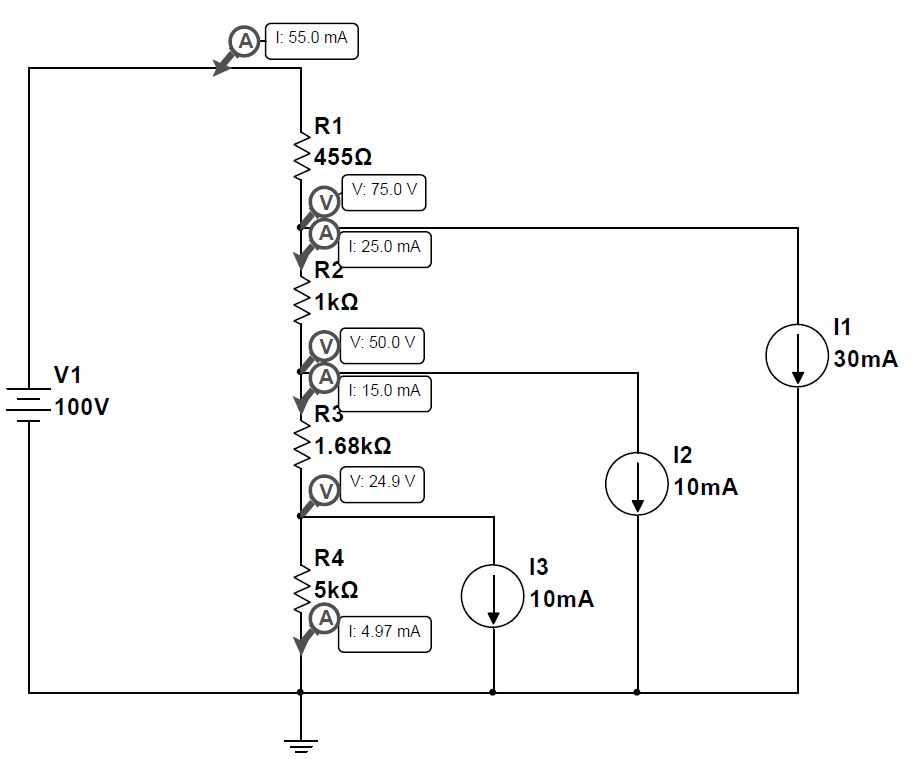
\includegraphics[scale=0.7]{figure7}
			\caption{Simulación del circuito para el ejemplo 3}
			\label{fig:pic7}
		\end{figure}
		
		Un punto importante en la determinación del resistor cuando se aplica la regla del 10 por ciento es que, para calcular la corriente de purga se debe tomar el 10\% de la carga total
		
		Encuentre la corriente de purga, la cual es el 10\% (0.1) de a corriente total
		\begin{equation}
			I_{R4} = (0.1)(10 mA + 10mA + 30mA) = 5mA\nonumber
		\end{equation} 
		
		Usamos la ley de Ohm para calcular $R_4$ (el resistor de purga)
		\begin{equation}
			R_4 = \frac{25V-0V}{0.005 A} = 5k\Omega \nonumber
		\end{equation}
		 
		La corriente a través de $R_3$ es igual a la corriente a través de $R_4$ más la corriente a través de la carga 3
		\begin{equation}
			I_{R3} = I_{R4} + I_{Load3} = 5mA + 10mA = 15mA\nonumber
		\end{equation} 
		 
		Para encontrar $R_3$ use la ley de Ohm usando la diferencia de voltaje entre la carga 2 y la carga 3
		\begin{equation}
			R_3 = \frac{50V - 25V}{0.015A} = 1667\Omega \nonumber
		\end{equation}
		O $1.68 k\Omega$ considerando las tolerancias y valores de resistencia estándar
		 
		La corriente a través de $R_2$ es
		\begin{equation}
			I_{R2} = I_{R3} + I_{Load2} = 15mA + 10mA = 25mA\nonumber
		\end{equation}
		 
		Usamos la ley de Ohm para calcular $R_2$
		\begin{equation}
			R_2 = \frac{75V - 50V}{0.025 A} = 1k\Omega\nonumber
		\end{equation} 
	
		La corriente a través de $R_1$ es
		\begin{equation}
			I_{R1} = I_{R2} + I_{Load1} = 25mA + 30mA = 55mA\nonumber
		\end{equation}
	
		Por último, usamos la ley de Ohm para calcular $R_1$
		\begin{equation}
			R_1 = \frac{100V - 75V}{0.055 A} = 455\Omega\nonumber
		\end{equation}
	\end{myexample}

	%\cite{textbook}
	\bibliographystyle{plain}
	\bibliography{citation.bib}
	
\end{document}